\chapter{Introduction}\label{chap:intro}
The existence of planets orbiting other stars different from our Sun, lived in the human imagination for centuries. During the sixteenth century, the Italian philosopher Giordano Bruno suggested, for the first time in history, that more planet could be outside the Solar System. Even though the first claims of exoplanet detection began at the end of the nineteenth century, it was not until more than four hundred years after the statement of Giordano Bruno, that the first exoplanet was confirmed in 1992. Surprisingly it was not just one exoplanet but three, orbiting the pulsar PSR B1257+12 more than 1000 light-years away from us. Today, more than 4,000 exoplanet are confirmed, and thousands more are waiting for their confirmation.

The increasing number of discovered exoplanets have been reach thanks to two techniques: Radial Velocity and Transits. Each one of these techniques had their own advantages depending on the physical properties of the planetary system. When the orbit of the exoplanet is aligned with the line of sight from Earth, the pass of the planet in front of its host star, the star's flux decreases proportionally to the size of the planet. Thus, its radius, in comparison with the radius of the star, can be determined directly using the Transit method. In the other hand, the gravity due to the presence of a planet will set the center of mass of the system, in a place different from the star's center. Therefore, the star will move in its own small orbit with a size proportional to the mass of the planet. In this case, the planet's minimum mass ($M_{p}\cdot \sin i$) can be determined. The perfect scenario comes when both method can be use in the same planetary system, allowing to derived essential properties as the real mass and the mean density of the planet.


\section{Transiting Exoplanets}
The Transit method is today the most successful technique to discover extrasolar planets. The Kepler mission was launched in 2009 and during its almost nine years of 
\begin{figure}[H]
\centering
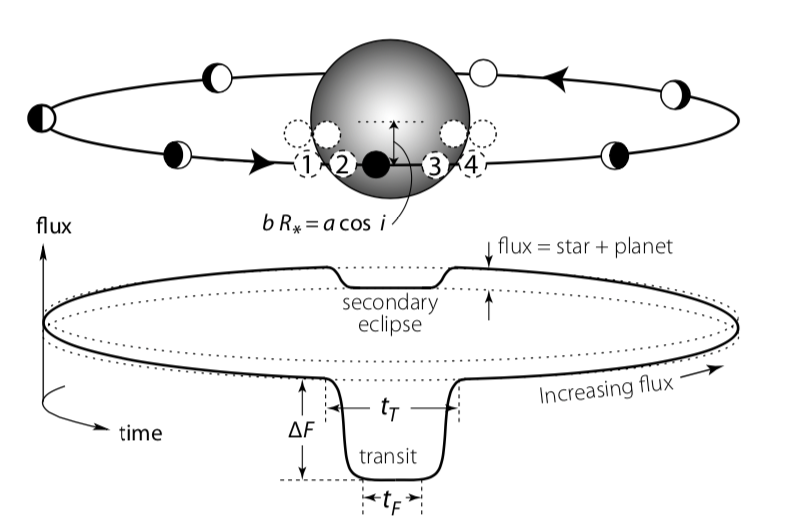
\includegraphics[width=0.8\columnwidth]{imagenes/transit.png}
\caption{Architecture of a transiting exoplanet.}
\label{transit}
\end{figure}

\begin{figure}[H]
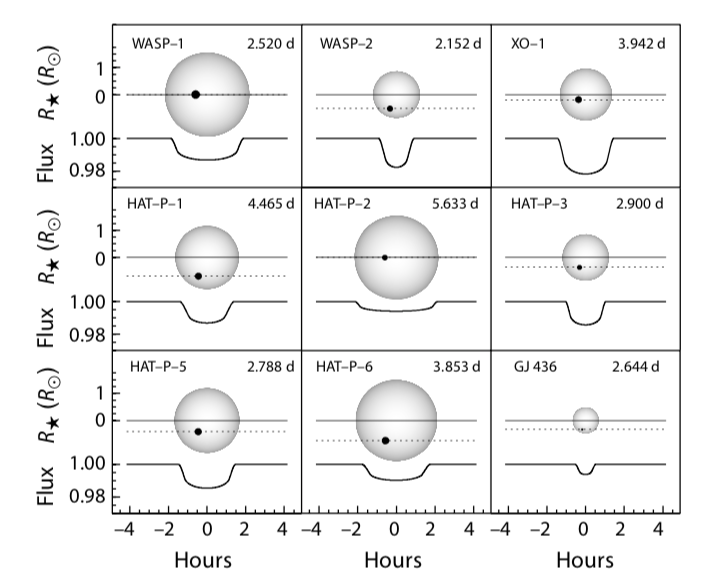
\includegraphics[width=1.0\columnwidth]{imagenes/transit_examples.png}
\caption{Examples of transiting exoplanets and how their light curves differ between them thanks to the physical properties of the exoplanet.}
\label{transit_examples}
\end{figure}



\section{Transit Timing Variations}

\section{The Transit Monitoring in the South project}